\documentclass[]{beamer}
\usepackage[T1]{fontenc}
\usepackage[utf8]{inputenc}
\usepackage{lmodern}
\usepackage[italian]{babel}
\usepackage{mathrsfs}
\usepackage{cancel}

\title{L'induzione elettromagnetica}
\author{\texorpdfstring{Mattia Cozzi\newline\href{mailto:cozzimattia@gmail.com}{\texttt{cozzimattia@gmail.com}}}{Mattia Cozzi}}
\date{a.s.~2023/2024}

%\documentclass[handout]{beamer}     %usare questa classe per generare l'handout
%\usepackage{pgfpages}   %per mostrare più quadri nella stessa pagina
%\pgfpagesuselayout{4 on 1}[a4paper,border shrink=5mm,landscape]
\usetheme{Singapore}
%\useoutertheme[left]{sidebar} %elementi intorno alle diapositive
\setbeamercovered{dynamic} %modifica l'aspetto del testo grigetto delle diapositive future. Argomenti: invisible/transparent/dynamic
\usecolortheme{orchid}
%COLORE PRINCIPALE
% \definecolor{marroncino}{RGB}{156, 26, 0} % UBC Blue (primary)
% \setbeamercolor{structure}{fg=marroncino} % itemize, enumerate, etc

\theoremstyle{plain}
\newtheorem{teorema}{Teorema}

\usepackage{tikz}
\usepackage{circuitikz}


\usepackage{pgf,pgfplots,graphicx}
\usetikzlibrary{angles,quotes,arrows,shapes,decorations.markings}
\pgfplotsset{compat=1.15}
\usepgfplotslibrary{units,fillbetween} % to add units easily to axis
\tikzset{fleche/.style args={#1:#2}{postaction=decorate,decoration={name=markings,mark=at position #1 with {\arrow[#2,scale=2]{>}}},},}

\newcommand{\fem}{f_{em}}
\newcommand{\femm}{f_{em0}}

\begin{document}

\begin{frame}
  \titlepage
\end{frame}





\begin{frame}
\frametitle{Contenuti}
\tableofcontents
\end{frame}


\section{Fenomeni induttivi}

\begin{frame}
  \frametitle{Magneti e correnti}
  Sappiamo che una corrente genera un campo magnetico (esperimento di \O rsted).\\~\\\pause
  \begin{block}{Domanda}
    Può un campo magnetico generare una corrente?
  \end{block}\pause
  ~\\Risposta positiva sarà data da Michael Faraday in Inghilterra e Joseph Henry negli Stati Uniti intorno al 1831.
\end{frame}







\begin{frame}
  \frametitle{Fenomeni induttivi (1)}
\begin{figure}
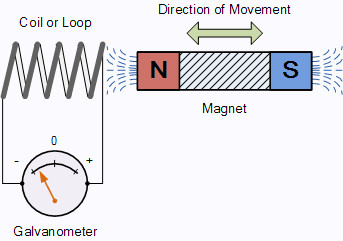
\includegraphics[width=.7\columnwidth]{img/induzione0.jpg}
\end{figure}
\end{frame}

\begin{frame}
  \frametitle{Fenomeni induttivi (2)}
\begin{figure}
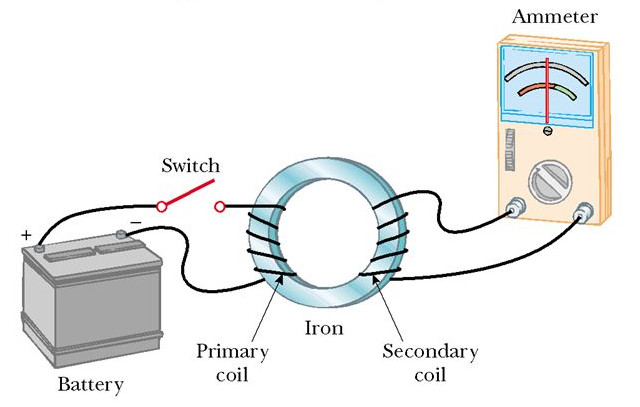
\includegraphics[width=.8\columnwidth]{img/induzione1.jpg}
\end{figure}
\end{frame}

\begin{frame}
  \frametitle{Fenomeni induttivi (3)}
\begin{figure}
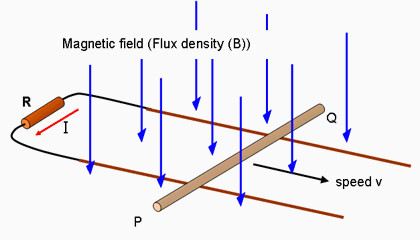
\includegraphics[width=.8\columnwidth]{img/induzione2.jpg}
\end{figure}
\end{frame}




\begin{frame}
  \frametitle{La variazione del flusso}
  Ricordando che:
\begin{center}
\colorbox{blue!30}{$ \Phi_S (\vec{B}) = \vec{B} \cdot \vec{S} = BS \cos\theta \quad [T \cdot m^2] = [Wb]$}
\end{center}\pause
possiamo affermare che  si ha una corrente indotta (causata da una forza elettromotrice indotta) ogniqualvolta si ha una variazione di flusso magnetico (causata da una variazione del campo, della superficie o dell'angolo che essi formano).\pause
\begin{block}{Causa della corrente indotta}
Si ha una corrente indotta quando varia il flusso del campo magnetico attraverso la superficie che ha per contorno il circuito indotto.
\end{block}
\end{frame}



\begin{frame}
\frametitle{Esercizi}
\begin{exampleblock}{Variazione del flusso (1)}
  \small{
  Una spira conduttrice circolare di raggio $ 2,4 \, cm $ è immersa in un campo magnetico uniforme di $ 90 \, \mu T $, inizialmente perpendicolare al piano della spira. Successivamente la spira ruota intorno al suo diametro con una velocità angolare costante di $ 10 \, rad/s $. Considera un intervallo di tempo di $ 0,010 \, s $.
  
  Calcola la variazione del flusso attraverso la spira.\hspace*{\fill}[$ -7,5 \times 10^{-8} \, Wb $]}
\end{exampleblock}

~

\begin{exampleblock}{Variazione del flusso (2)}
  \small{
  Una sbarra conduttrice chiude un circuito a forma di U, immerso in un campo magnetico  di $ 0,40 \, T $ diretto perpendicolarmente alla superficie del circuito. La sbarra, lunga $ 10 \, cm $, viene spostata alla velocità di $ 3,0 \, cm/s $ per un intervallo di $ 3,0 \, s $.

  Calcola variazione di flusso nell'intervallo di tempo dato.\hspace*{\fill}[$ \pm 3,6 \times 10^{-3} \, Wb $]}
\end{exampleblock}
\end{frame}

\section{Faraday-Neumann-Lenz}


\begin{frame}
  \frametitle{Espressione matematica del legame tra $ fem_{ind} $ e flusso}
\begin{block}{Legge di Faraday-Neumann}
\[ fem_{ind} = - \frac{\Delta \Phi(\vec{B})}{\Delta t} \]\pause
Per la forza elettromotrice indotta istantanea:
\[ fem_{ist} = \lim_{\Delta t \rightarrow 0} \left( - \frac{\Delta \Phi(\vec{B})}{\Delta t} \right) = - \frac{d \Phi(\vec{B})}{d t} \]
\end{block}\pause
\begin{alertblock}{Attenzione}
La forza elettromotrice indotta istantanea è la derivata temporale del flusso del campo magnetico cambiata di segno.
\end{alertblock}
\end{frame}

\begin{frame}
  \frametitle{Il campo magnetico indotto}
  La variazione di flusso genera una corrente indotta.\pause

  ~
  
  La corrente indotta genera un campo magnetico ``indotto''.\pause

  ~
  
  Questo ``campo magnetico indotto'' può:
  \begin{itemize}
    \item rafforzare la variazione del campo esterno;\pause
    \item contrastare la variazione del campo esterno.\pause
  \end{itemize}
  \alert{La seconda opzione è l'unica possibile}: se la variazione venisse rafforzata, si genererebbe una corrente indotta ancora più intensa, che rafforzerebbe di nuovo la variazione, in un circolo infinito. Tutto ciò è in contrasto con il principio di conservazione dell'energia.
\end{frame}

\begin{frame}
  \frametitle{La legge di Lenz}
  \begin{block}{Legge di Lenz}
    Il verso della corrente indotta è sempre tale da \emph{opporsi alla variazione} di flusso che la genera.\pause
  \end{block}

  ~

  La legge di Lenz è espressa dal segno ``$ - $'' della legge di Faraday-Neumann (Legge di Faraday-Neumann-Lenz).
\end{frame}




\begin{frame}
\frametitle{Esercizi}
\begin{exampleblock}{Calcolo della corrente indotta}
  \small{
  Facendo riferimento alla sbarra conduttice dell'esercizio \textbf{Variazione del flusso (2)}, calcola la corrente che circola nel circuito a causa dello spostamento della sbarra, sapendo che il circuito ha una resistenza di $ 5,0 \, \Omega $.\hspace*{\fill}[$ -7,5 \times 10^{-8} \, Wb $]}
\end{exampleblock}

~

\begin{exampleblock}{Lavorare con le funzioni}
  \small{
    Una spira di area $ S = 0,35 \, m^2 $ ha resistenza elettrica $ R = 70 \, \Omega $ ed è attraversata da un campo magnetico perpendicolare al piano di $ S $. A partire dall’istante $ t_0 = 0 \, s $ il campo inizia a variare secondo la legge:
    \begin{center}
      $ B(t) = B_0 \cos (\omega t) $
    \end{center}
    con $ B_0 = 2,0 \times 10^{-2} \, T  $ e $ \omega = \pi \, \frac{rad}{s} $ e $ t $ in secondi.
    
    Esprimi l’intensità della corrente indotta nella spira in funzione di $ t $. Qual è il valore massimo di tale corrente per $ t \geq 0 $?}
\end{exampleblock}
\end{frame}


\section{Autoinduzione}

\begin{frame}
\frametitle{Autoinduzione in un circuito}
Per avere fenomeni induttivi non è necessario un campo magnetico \emph{esterno}.\pause

\begin{columns}
\begin{column}{.55\textwidth}
  Una corrente variabile in un circuito genera un campo magnetico variabile, che genera a sua volta una $ \fem $ indotta nel circuito stesso.\pause

~

Tale fenomeno è noto con il nome di \alert{autoinduzione}, e si presenta per un tempo molto breve all'apertura e alla chiusura di un circuito (oppure in regime di corrente alternata).
\end{column}
\begin{column}{.35\textwidth}
  \begin{figure}
    \visible<3->{\begin{figure}
      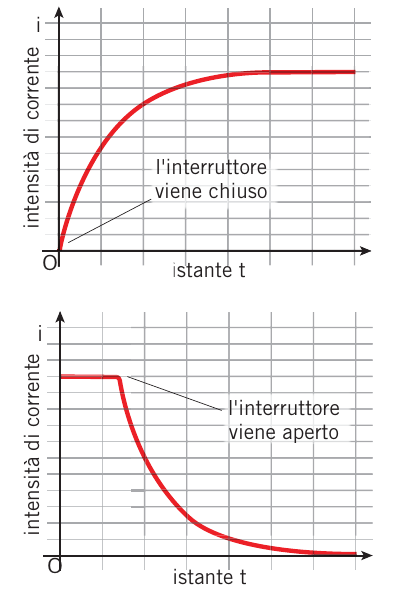
\includegraphics[width=\columnwidth]{img/aperturachiusura.png}
    \end{figure}}
  \end{figure}
\end{column}
\end{columns}
\end{frame}



\begin{frame}
  \frametitle{Induttanza}
  Maggiore è la corrente di un circuito, maggiore è il flusso del campo magnetico che attraversa il circuito stesso: \alert<1>{flusso magnetico e corrente sono direttamente proporzionali}.\pause
  
  ~
  
  Possiamo esprimere questo fatto con la formula:
  \begin{center}
\colorbox{blue!30}{$ \Phi (\vec{B}) = Li $}
\end{center}\pause
Il valore della costante di proporzionalità $ L $ (induttanza del circuito, misurata in \emph{henry}) dipende da come e da quali materiali è costituito il circuito.
\begin{center}
$ \left[ H \right] = \left[ \dfrac{Wb}{A} \right] $
\end{center}
\end{frame}

\begin{frame}
\frametitle{Induttanza}
\begin{columns}
\begin{column}{.5\textwidth}
  \begin{figure}
    \ctikzset{bipoles/length=1.2cm}
    \begin{circuitikz}[scale=0.5]
    \draw (0,0) to[L, l=$L$] (8,0);
    \draw (4,-3) to[battery1](8,-3);
    \draw (0,-3) to[R] (4,-3);
    \draw (0,0) to[short] (0,-3);
    \draw (8,0) to[short] (8,-3);
    \end{circuitikz}
  \end{figure}
\end{column}
\begin{column}{.3\textwidth}
    \begin{figure}
      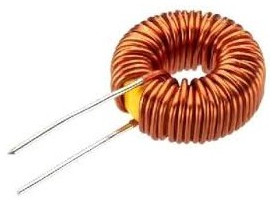
\includegraphics[width=.8\columnwidth]{img/induttanza.jpg}
    \end{figure}
\end{column}
\end{columns}

~

~

In un circuito, il simbolo indica il fenomeno dell'induttanza in sé o una bobina inserita nel circuito per amplificare l'effetto dell'autoinduzione.
\end{frame}


\begin{frame}
\frametitle{Esercizio}
\begin{exampleblock}{Calcolo della $\fem$}
  \small{
  Un circuito ha un coefficiente di autoinduzione di $ 5,5 \times 10^{-1} \, H $. L'intensità di corrente passa da $ 0 $ a $ 5,0 \times 10^{-1} \, A $ in un tempo di $ 4,0 \, s $.
  
  Calcola la $\fem$ indotta nel circuito.\hspace*{\fill}[$ -69 \, mV $]}
\end{exampleblock}
\end{frame}

\begin{frame}
\frametitle{Circuito RL}
Come si comporta la corrente in presenza di induttanza?
\begin{columns}
\begin{column}{0.5\textwidth}
\visible<1->{\begin{figure}\centering
\ctikzset{bipoles/length=1.2cm}
\begin{circuitikz}[scale=0.7]
\draw (6,0) to[switch] (0,0);
\draw (0,4) to[battery1, l=$\Delta V$] (0,0);
\draw (0,4) to[R, l=R] (6,4);
\draw (6,4) to[L, a_=$L$] (6,0);
\end{circuitikz}
\end{figure}}
\end{column}
\begin{column}{0.5\textwidth}
\visible<2->{~\\~\\Alla chiusura del circuito: \begin{center}
\colorbox{blue!30}{$ i(t) = \dfrac{\Delta V}{R} \cdot \left( 1 - e^{-\frac{R}{L}t} \right) $}
\end{center}}
\visible<3->{~\\~\\All'apertura del circuito: \begin{center}
\colorbox{blue!30}{$ i(t) = \dfrac{\Delta V}{R} \cdot e^{-\frac{R}{L}t}  $}
\end{center}}
\end{column}
\end{columns}

~

\visible<4>{Definiamo per comodità la \alert{costante di tempo del circuito RL}:
\begin{center}
  $ \tau = \dfrac{L}{R} $
\end{center}}
\end{frame}


\begin{frame}
\frametitle{Grafici di $ i(t) $ nel circuito RL}
\begin{columns}
\begin{column}{.4\textwidth}
  \begin{figure}
  Alla chiusura:

  ~

  \begin{tikzpicture}[xscale=.4,yscale=1.2]
  \node [left] at (0,1) {{\scriptsize $ i_0 = \frac{\Delta V}{R} $}};
  \node [left] at (0,2) {{\scriptsize $ i(t) \, [A] $}};
  \node [below] at (7,0) {{\scriptsize $ t \, [s] $}};
  \draw [->] (-1,0) -- (7,0);
  \draw [->] (0,-.1) -- (0,2);
  \draw[smooth, blue, thick, domain=0:6] plot (\x,{1 - e^(-\x)});
  \draw[smooth, dashed, domain=0:6] plot (\x,{1});
  \end{tikzpicture}

  ~

  $ i(t) = \frac{\Delta V}{R} \cdot \left( 1 - e^{-\frac{t}{\tau}} \right) $

  ~

  $ \displaystyle \lim_{ t \rightarrow + \infty} i(t) = i_0 $
  \end{figure}
\end{column}
\begin{column}{.4\textwidth}
  \begin{figure}
  All'apertura:

  ~

  \begin{tikzpicture}[xscale=.4,yscale=1.2]
  \node [left] at (0,1) {{\scriptsize $ i_0 = \frac{\Delta V}{R} $}};
  \node [left] at (0,2) {{\scriptsize $ i(t) \, [A] $}};
  \node [below] at (7,0) {{\scriptsize $ t \, [s] $}};
  \draw [->] (-1,0) -- (7,0);
  \draw [->] (0,-.1) -- (0,2);
  \draw[smooth, red, thick, domain=2:6] plot (\x,{e^(-\x + 2)});
  \draw[smooth, red, thick, domain=0:2] plot (\x,{1});
  \end{tikzpicture}

  ~

  $ i(t) = \frac{\Delta V}{R} \cdot e^{-\frac{t}{\tau}}  $

  ~

  $ \displaystyle \lim_{ t \rightarrow + \infty} i(t) = 0 $
  \end{figure}
\end{column}
\end{columns}
\end{frame}



\begin{frame}
\frametitle{Esercizio}
\begin{exampleblock}{Circuito RL}
  \small{
    Un circuito RL contiene un generatore con una tensione di $ 10 \, V $, una resistenza da $ 6,2 \, \Omega $ e una bobina con induttanza $ 1,5 \, H $.

    \begin{itemize}
      \item Calcola il valore di $ i_0  $, cioè il valore a cui tende $ i(t) $ a circuito chiuso.\hspace*{\fill}[$ 1,6 \, A $]
      \item Calcola dopo quanto tempo dall'apertura del circuito l'intensità di corrente è il $ 10\% $ di $ i_0 $.\hspace*{\fill}[$ 0,56 \, s $]
      \item Determina il valore di $ i $ dopo un tempo $ t = L/R $.\hspace*{\fill}[$ i = i_0 / e $]
    \end{itemize}}
\end{exampleblock}
\end{frame}



\begin{frame}
\frametitle{$ \fem $ nel circuito RL}
In un circuito RL avremo una corrente variabile, e pertanto ci sarà una variazione di flusso:

\begin{center}
  $ \Delta \Phi(\vec{B}) = \Phi_2 - \Phi_1 = Li_2 - Li_1 = L\Delta i $\pause
\end{center}

La variazione di flusso genera una $ \fem $ indotta, il cui valor medio è:\pause
\begin{center}
$ \fem = - \dfrac{\Delta\Phi}{\Delta t} = -L \dfrac{\Delta i}{\Delta t} $\pause
\end{center}
\begin{block}{Forza elettromotrice con induttanza}
La $ \fem $ istantanea in un circuito con induttanza è:
\begin{center}
  \colorbox{blue!30}{$ \displaystyle f_{em \, ist} = \lim_{\Delta t \rightarrow 0} - \dfrac{\Delta\Phi}{\Delta t} = \lim_{\Delta t \rightarrow 0} -L \dfrac{\Delta i}{\Delta t} = - L \dfrac{d i}{d t} = - Li'(t)  $}
\end{center}
\end{block}  
\end{frame}


\section{Corrente alternata}

\begin{frame}
  \frametitle{L'alternatore}
  
  \visible<1->{\begin{block}{Alternatore}
Un alternatore è un dispositivo che trasforma energia cinetica in energia elettrica.
\end{block}}
\visible<2->{È costituito da una spira che viene fatta ruotare con velocità angolare costante all'interno di un campo magnetico. La variazione di flusso magnetico genera una corrente indotta.
\begin{columns}
\begin{column}{0.3\textwidth}
\begin{figure}
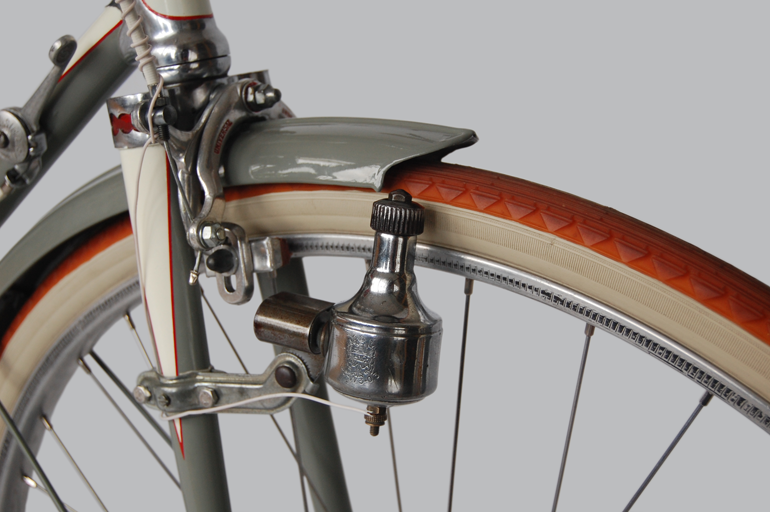
\includegraphics[width=\columnwidth]{img/alternatore1.png}
\end{figure}
\end{column}
\begin{column}{0.3\textwidth}
\begin{figure}
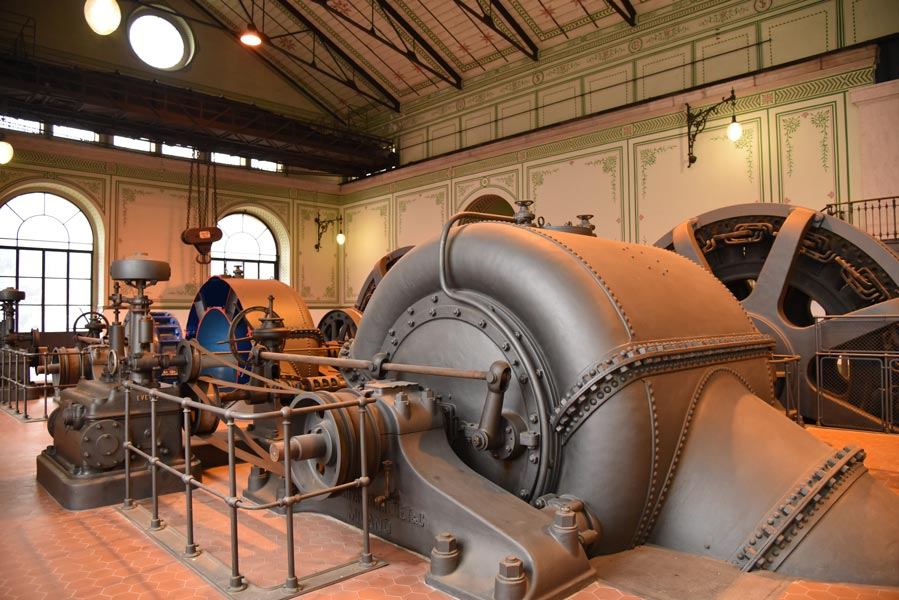
\includegraphics[width=\columnwidth]{img/alternatore2.jpg}
\end{figure}
\end{column}
\begin{column}{0.3\textwidth}
\begin{figure}\centering
\ctikzset{bipoles/length=1.5cm}
\begin{circuitikz}[scale=0.5]
\draw (0,0) to[vco, *-*] (4,0);
\end{circuitikz}
\end{figure}
\end{column}
\end{columns}}
\end{frame}



\begin{frame}
  \frametitle{Schema di un alternatore}
  \begin{figure}
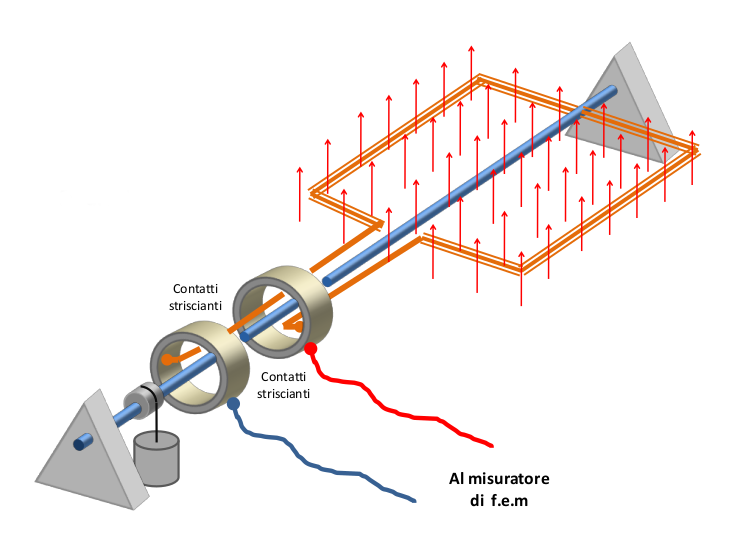
\includegraphics[width=0.8\columnwidth]{img/alternatore.png}
\end{figure}
\end{frame}


\begin{frame}
  \frametitle{Calcolo della $ \fem $ alternata (1)}
  Se la spira ruota con velocità angolare costante $ \omega $, allora l'angolo $ \theta $ tra il campo magnetico e il vettore normale alla spira varia secondo la relazione:
\begin{center}
$ \theta = \omega t $
\end{center}\pause
  Esprimeremo allora il flusso del campo magnetico \emph{in funzione del tempo} con:
  \begin{center}
$ \Phi (\vec{B}) = BS \cos\theta = BS\cos(\omega t) $
\end{center}
  \pause
  Possiamo calcolare la $ \fem $ indotta nella spira con la legge di Faraday-Neumann-Lenz (derivando cioè in funzione del tempo).
\end{frame}




\begin{frame}
  \frametitle{Calcolo della $ \fem $ alternata (2)}
  \begin{center}
$ \fem (t) = - \dfrac{d \Phi (\vec{B})}{dt} = - \dfrac{d(BS\cos(\omega t))}{dt} = BS\omega\cdot\sin(\omega t) $
\end{center}\pause
  Il coefficiente $ BS\omega $ rappresenta l'ampiezza dell'oscillazione.\pause
  
  ~
  
  Ponendo $ BS\omega = \femm $ otteniamo:
  \begin{center}
\colorbox{blue!30}{$ \fem (t) = \femm \cdot \sin (\omega t) $}
\end{center}\pause
  Inoltre, ponendo $ i_0 = \dfrac{\femm}{R} $ avremo:
  \begin{center}
\colorbox{blue!30}{$ i (t) = i_0 \cdot \sin (\omega t) $}
\end{center}
\end{frame}

\begin{frame}
\frametitle{Grafico della corrente alternata}
\begin{figure}
  \begin{tikzpicture}[xscale=.4,yscale=1]
\node [left] at (0,1) {{\scriptsize $ i_0 $}};
\node [left] at (0,-1) {{\scriptsize $ - i_0 $}};
\node [above] at (1.5*pi,1) {{\scriptsize $ T = \dfrac{1}{f} $}};
\draw [->] (-4,0) -- (4*pi,0);
\node [below] at (4*pi,0) {{\scriptsize $ t \, [s] $}};
\node [left] at (0,2) {{\scriptsize $ i(t) \, [A] $}};
\draw [|<->|, dashed, thick] (.5*pi,1) -- (2.5*pi,1);
\draw [-, dotted] (.5*pi,1) -- (0*pi,1);
\draw [-, dotted] (0*pi,-1) -- (1.5*pi,-1);
\draw [->] (0,-2) -- (0,2);
\draw[smooth, red, thick, domain=-pi:3.5*pi] plot (\x, {sin(\x r)});
\end{tikzpicture}
\end{figure}

~

Valgono, come per ogni onda, le relazioni $ T = \dfrac{2 \pi}{\omega} $ e \colorbox{blue!30}{$ f = \dfrac{\omega}{2\pi} $}.\pause

~

In Europa $ f = 50 \, Hz $, mentre negli Stati Uniti $ f = 60 \, Hz $.
\end{frame}




\begin{frame}
\frametitle{Potenza media in corrente alternata}
Ricordiamo che, in corrente continua, $ P = i^2 R = i \Delta V $.\pause

~

\alert<2>{La potenza in regime di corrente alternata} è una funzione del tempo ed \alert<2>{ha sempre segno positivo} anche se la corrente cambia verso ad ogni periodo.
  
  \begin{columns}
\begin{column}{0.25\textwidth}
  $ P(t) = R i^2(t) $
\end{column}
\begin{column}{0.55\textwidth}
\visible<2->{\begin{figure}
\begin{tikzpicture}[xscale=.6,yscale=1.5]
\node [left] at (0,1) {{\tiny $ R i_0^2 $}};
\node [left] at (0,1.5) {{\tiny $ P(t) \, [W] $}};
\node [below] at (7,0) {{\tiny $ t \, [s] $}};
\node [left] at (0,.5) {{\tiny $ \frac{1}{2}R i_0^2 $}};
\draw [->] (-.5,0) -- (7,0);
\draw [-, dotted] (0,1) -- (7,1);
\draw [-, dashed, thick] (0,0.5) -- (7,0.5);
\draw [->] (0,-.2) -- (0,1.5);
\draw[smooth, samples=100, red, thick, domain=0:7] plot 
(\x, {sin(\x r)*sin(\x r)});
\end{tikzpicture}
\end{figure}}
\end{column}
\end{columns}\pause

~

La \alert<3>{potenza media} erogata sarà \colorbox{blue!30}{$ \overline{P} = \dfrac{1}{2}R i_0^2 $}.
\end{frame}



\begin{frame}
\frametitle{Valori efficaci}
  La medesima potenza sarebbe erogata in regime di corrente continua se nel circuito passasse una corrente detta \emph{corrente efficace}:
  \begin{center}
  $ \dfrac{1}{2}R i_0^2 = R i_{eff}^2 $
  \end{center}\pause
  e pertanto:
  \begin{center}
\colorbox{blue!30}{$ i_{eff} = \dfrac{i_0}{\sqrt{2}} $}~~~ e inoltre ~~~\colorbox{blue!30}{$ f_{eff} = \dfrac{\femm}{\sqrt{2}} $}
\end{center}\pause

~

La potenza media erogata sarà allora \colorbox{blue!30}{$ \overline{P} = i_{eff} f_{eff} $}.\pause

~

Quando diciamo che nei circuiti domestici la $ \fem $ è di $ 220 \, V $ intendiamo che $ f_{eff} = 220 \, V $.
\end{frame}



\begin{frame}
\frametitle{Esercizio}
\begin{exampleblock}{Circuito in corrente alternata}
  \small{
    Un generatore fornisce una tensione alternata con valore massimo di $ 80 \, V $ e frequenza $ 50 \, Hz $. Il circuito ha una resistenza totale di $ 15 \, \Omega $.

    \begin{itemize}
      \item Calcola il valore massimo della corrente che attraversa il resistore.\hspace*{\fill}[$ 5,3 \, A $]
      \item Determina l'equazione che esprime l'andamento della tensione alternata in funzione del tempo.
    \end{itemize}}
\end{exampleblock}
\end{frame}



\begin{frame}
\frametitle{Esercizio}
\begin{exampleblock}{Energia dissipata}
  \small{
    Un generatore di tensione alternata è collegato ad una stufa di resistenza $ 250 \, \Omega $. Il valore massimo della tensione alternata è di $ 200 \, V $. Calcola:

    \begin{itemize}
      \item il valore efficace della corrente;\hspace*{\fill}[$ 0,566 \, A $]
      \item la potenza dissipata dalla stufa;\hspace*{\fill}[$ 80,0 \, W $]
      \item il calore dissipato per effetto Joule in un tempo di $ 15 \, min $.\hspace*{\fill}[$ 7,20 \times 10^{4} \, J $]
    \end{itemize}}
\end{exampleblock}
\end{frame}




\section{Trasformatore}



\begin{frame}
\frametitle{Il trasformatore}
\begin{block}{Definizione}
  Il trasformatore è un dispositivo che sfrutta l'induzione elettromagnetica per modificare il valore della $ \fem $ e della corrente in regime alternato.
\end{block}


\visible<2->{
\begin{columns}
\begin{column}{0.45\textwidth}
È composto da un nucleo di ferro, intorno al quale si trovano avvolte due bobine con un numero di avvolgimenti diversi.
\end{column}
\begin{column}{0.5\textwidth}
\begin{figure}
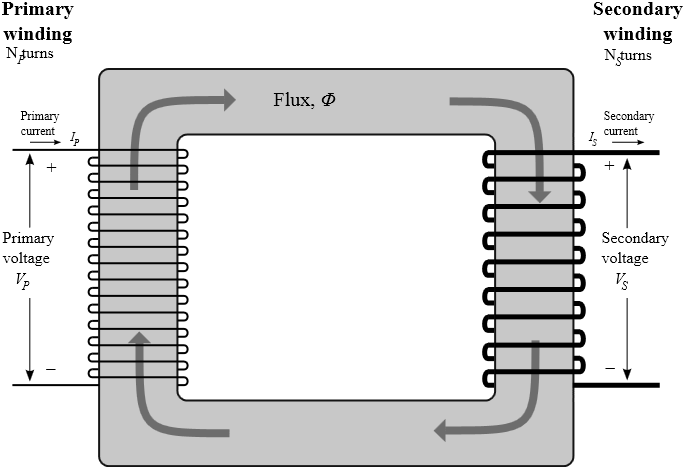
\includegraphics[width=\columnwidth]{img/trasformatore.png}
\end{figure}
\end{column}
\end{columns}}
\end{frame}


\begin{frame}
\frametitle{Relazioni tra i valori efficaci}
Indicando con $ f_{eff1} $ la tensione efficace in ingresso (avvolgimento con $ n_1 $ spire) e con $ f_{eff2} $ la tensione in uscita, la legge di FNL ci permette di affermare:
\begin{center}
\colorbox{blue!30}{$ \dfrac{f_{eff2}}{n_2} = \dfrac{f_{eff1}}{n_1} $}
\end{center}\pause
Il rapporto $ \dfrac{n_2}{n_1} $ è detto \alert<2>{rapporto di trasformazione}.\pause

~

Per un trasformatore ideale (cioè in cui la potenza in ingresso sia uguale alla potenza in uscita) vale inoltre:
\begin{center}
\colorbox{blue!30}{$ i_{eff2} f_{eff2} = i_{eff1} f_{eff1} $}
\end{center}
\end{frame}


\begin{frame}
\frametitle{Esempi}

\begin{columns}
\begin{column}{0.45\textwidth}
\begin{figure}
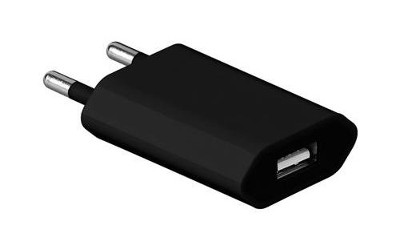
\includegraphics[width=0.8\columnwidth]{img/trasformatore1.jpg}

Input $ 220 \, V $, output $ 5 \, V $
\end{figure}
\end{column}
\begin{column}{0.45\textwidth}
\begin{figure}
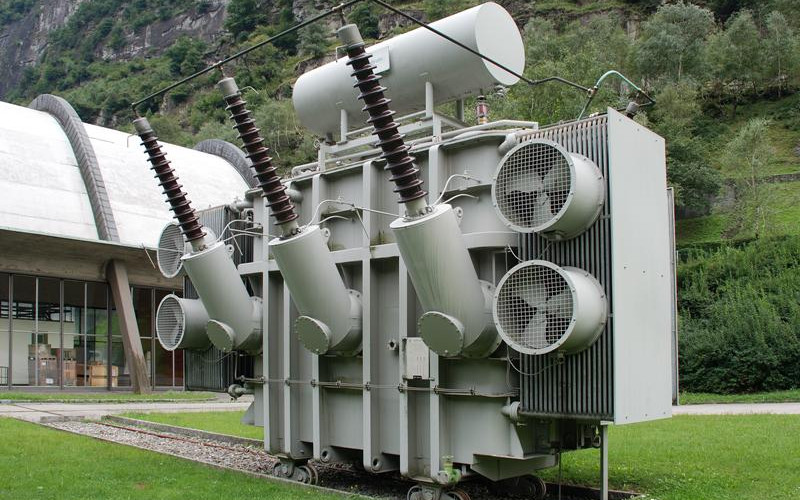
\includegraphics[width=0.8\columnwidth]{img/trasformatore2.jpg}

Input $ 132 \, kV $, output $ 15 \, kV $
\end{figure}
\end{column}
\end{columns}
\end{frame}





\begin{frame}
\frametitle{Esercizio}
\begin{exampleblock}{Trasformatore ideale e reale}
  \small{
    Il circuito primario di un trasformatore ha 140 spire, mentre il secondario ne ha 660. Al primario viene applicata una tensione di $ 220 \, V $ che genera una corrente di $ 15,0 \, A $.

    \begin{itemize}
      \item Calcola la corrente del secondario trascurando la dissipazione di energia.\hspace*{\fill}[$ 3,18 \, A $]
      \item Il trasformatore ha un rendimento del $ 95\% $. Calcola la sua potenza reale.\hspace*{\fill}[$ 3,1 \times 10^{3} \, W $]
    \end{itemize}}
\end{exampleblock}
\end{frame}


\end{document}
